\section{Results}
\label{sec:analysis}

The detailed accuracy and agreement results are presented in Table \ref{pelvis:resultsperrgait} and Figure \ref{blandaltman}. The pelvis roll angle in a stride (average of all strides of subjects) has been plotted in Figures \ref{fig:walk} and \ref{fig:trot} for both methods and both measurement devices. 

The results demonstrate a high level of accuracy of \gls{imu} for measuring pelvis roll angle. However, the agreement between the methods was low, for both of the measurement devices. During the walk, the pelvis roll angle calculation accuracy of a single \gls{imu} on the sacrum was 0.33 degrees compared to the rigid triad of markers. In the case of two \gls{imu}s on the tuber coxae, the accuracy was slightly higher resulting at 0.28 degrees when compared to the tuber coxae markers. 

The \gls{rmse} between methods using \gls{imu} was 2.09 degrees. However, this figure reduced to 1.57 degrees when employing the marker-based method. In addition, the accuracy of \gls{imu} on each method during trot was 0.67 degrees for single \gls{imu} calculation and 0.43 degrees for double \gls{imu} calculation. Using \gls{imu} as the measuring device, we achieved 3.59 degrees \gls{rmse} between methods while we calculated 3.55 degrees by using markers.


\begin{table}[!htbp] 
    \centering
    \caption{Accuracy and differences of the methods and the measurement devices outputs using \gls{rmse}. On each row, it is indicated that the \gls{rmse} presents the difference between the methods or measurement devices}% Add 'table' caption

    
    \resizebox{0.8\linewidth}{!}{% 
    
    \begin{tabular}{p{1cm}p{3cm}p{3.5cm}c}
    
    \midrule
    

     Gait &  Methods & Measurement devices & \gls{rmse} (degree) \\
     


        \midrule
        
Walk & Roll and Inverse sine &  \gls{imu} & 2.09\\[0.4 em]
    
Walk & Roll and Inverse sine &  \gls{omc} & 1.57\\[0.4 em]

Walk & Roll &  \gls{imu} and \gls{omc} & 0.33\\[0.4 em]

Walk & Inverse sine &  \gls{imu} and \gls{omc} & 0.28\\[0.4 em]

Trot & Roll and Inverse sine &  \gls{imu} & 3.59\\[0.4 em]
    
Trot & Roll and Inverse sine &  \gls{omc} & 3.55\\[0.4 em]

Trot & Roll &  \gls{imu} and \gls{omc} & 0.67\\[0.4 em]

Trot & Inverse sine &  \gls{imu} and \gls{omc} & 0.43\\[0.4 em]
    
        \bottomrule
    \end{tabular}}
        
    \label{pelvis:resultsperrgait}
    \end{table}

\begin{figure}[htbp]
\centering
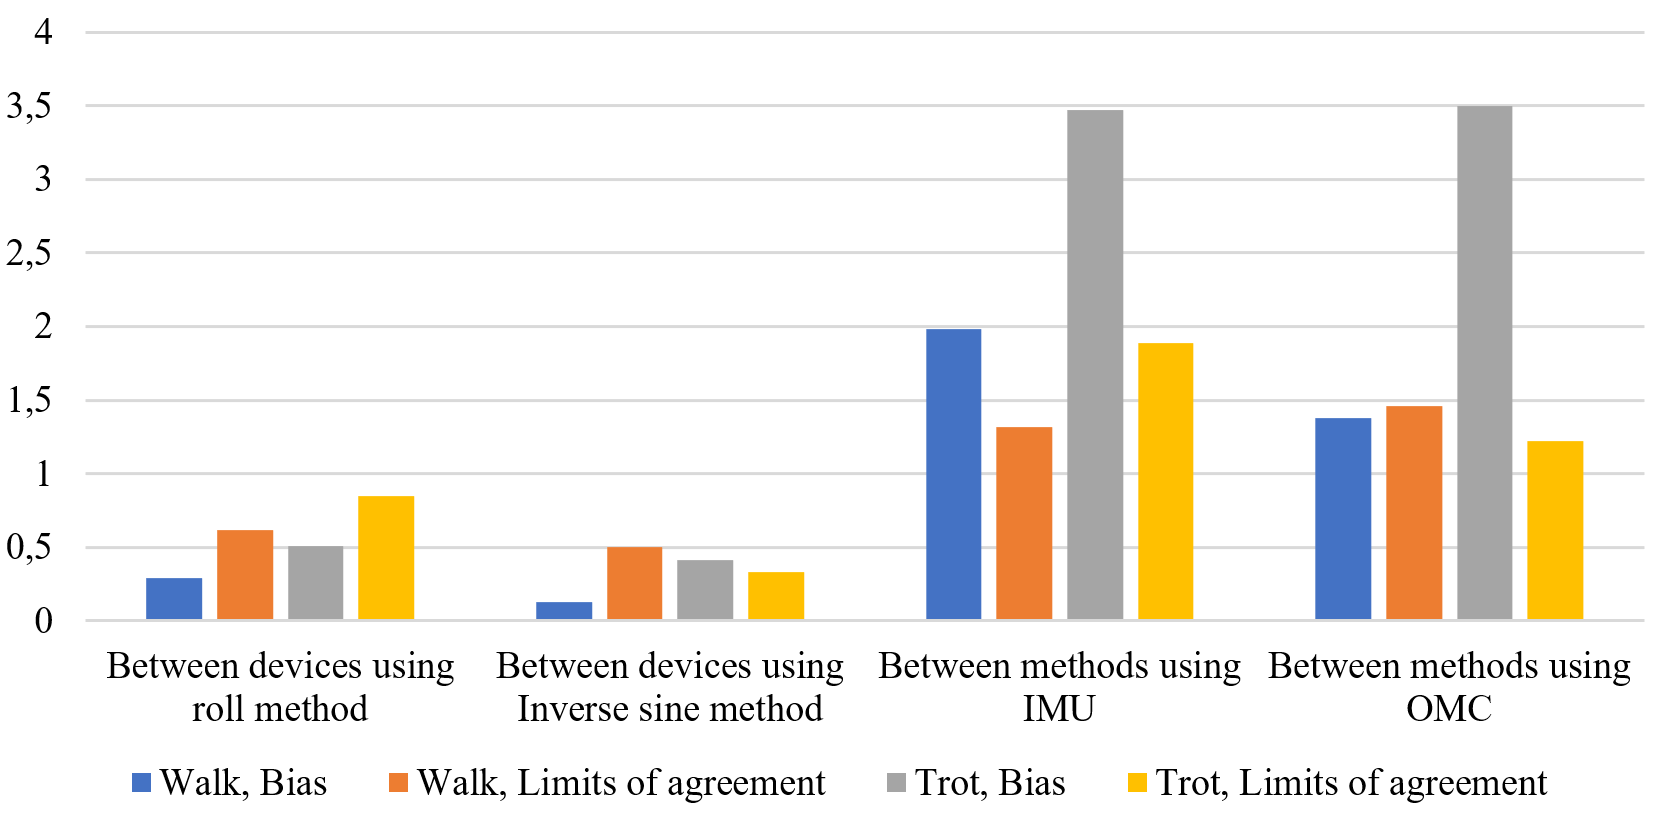
\includegraphics[width=\linewidth]{chapters/Pelvis/figures/Picture1.png}
\caption{Results from Bland-Altman analysis. The vertical axis is the measurement bias and limits of agreement}
\label{blandaltman}
\end{figure}

\begin{figure}[htbp]
\centering
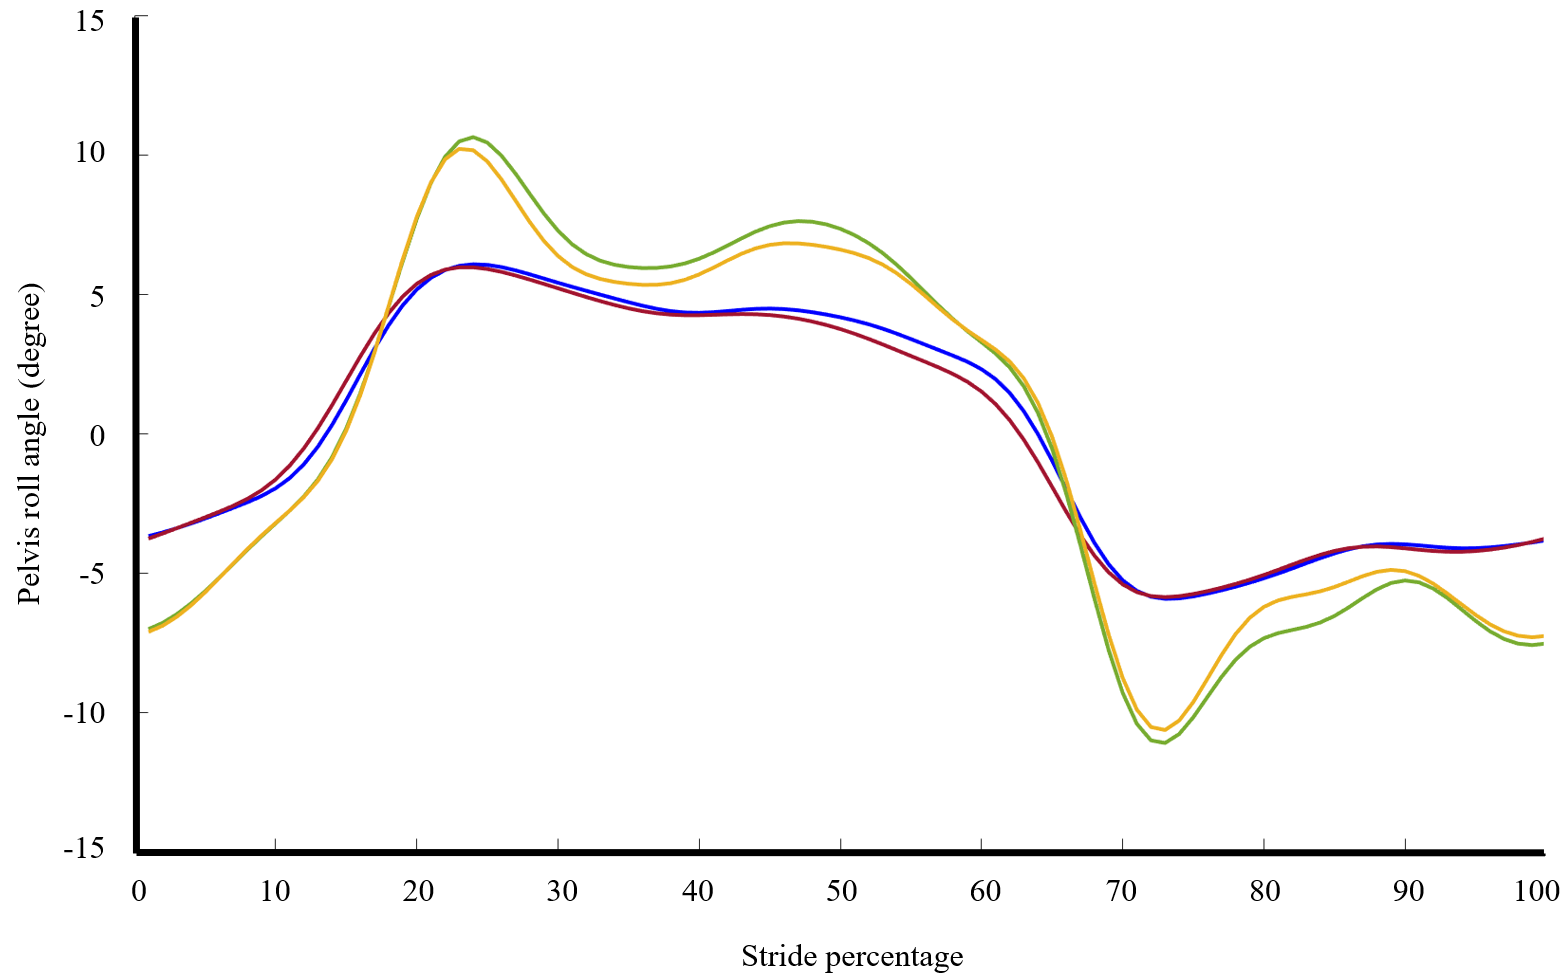
\includegraphics[width=.95\linewidth]{chapters/Pelvis/figures/PR.png}
\caption{Pelvis roll angle of a stride during walk (average of all subjects). Blue: Inverse sine method using \gls{omc}. Red: Inverse sine method using \gls{imu}. Green: Roll method using \gls{imu}. Yellow: Roll method using \gls{omc}.}
\label{fig:walk}
\end{figure}

\begin{figure}[htbp]
\centering
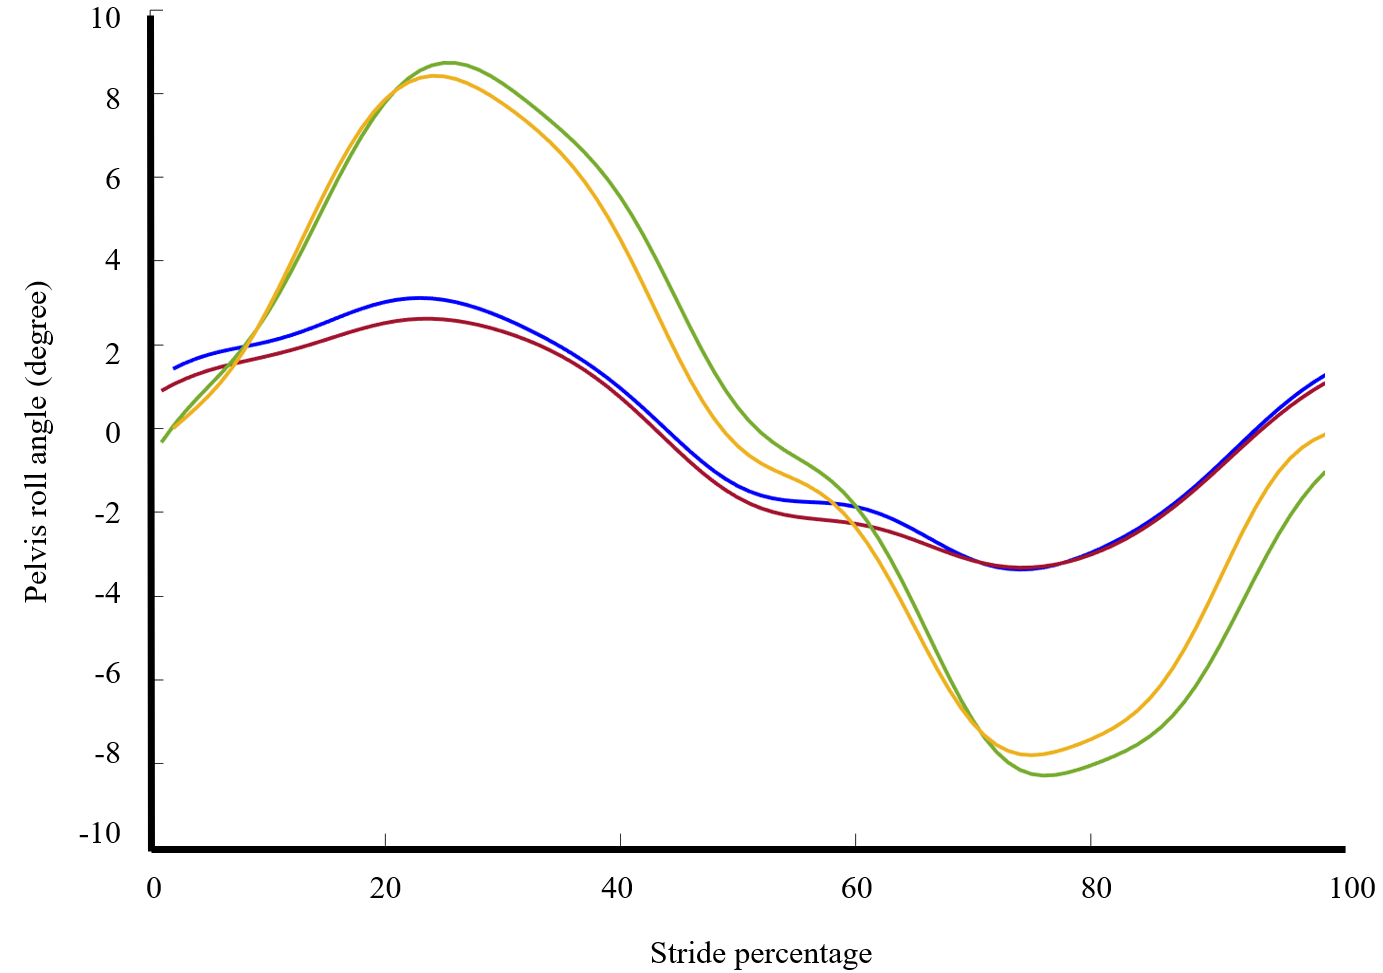
\includegraphics[width=.95\linewidth]{chapters/Pelvis/figures/PRtrot.png}
\caption{Pelvis roll angle of a stride during trot (average of all subjects). Blue: Inverse sine method using \gls{omc}. Red: Inverse sine method using \gls{imu}. Green: Roll method using \gls{imu}. Yellow: Roll method using \gls{omc}.}
\label{fig:trot}
\end{figure}